\documentclass{standalone}
\usepackage{amssymb} % мат. символы
    \DeclareMathSymbol{\sm}{\mathbin}{AMSa}{"39} % короткий минус
    \newcommand{\mo}{\sm\!1}
\usepackage{tikz}
    \usetikzlibrary{arrows.meta}
    \usetikzlibrary{calc}
\tikzset{gdst/.style=
    {circle, draw=black!50, very thick, minimum height=1.2cm, inner sep=2pt, text centered, }, }

\begin{document}
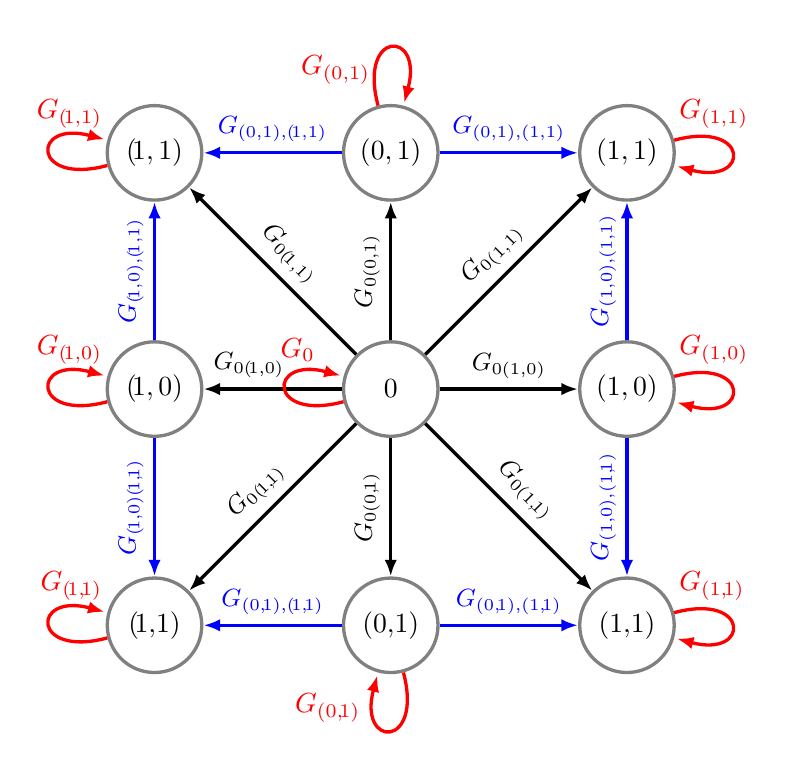
\begin{tikzpicture}
    \node[gdst, shift={(0,0)}] (f1) {${(\mo,\mo)}$};
    \node[gdst, shift={(3,0)}] (f2) {${(0,\mo)}$};
    \node[gdst, shift={(6,0)}] (f3) {${(1,\mo)}$};
    \node[gdst, shift={(0,3)}] (f4) {${(\mo,0)}$};
    \node[gdst, shift={(3,3)}] (f5) {${0}$};
    \node[gdst, shift={(6,3)}] (f6) {${(1,0)}$};
    \node[gdst, shift={(0,6)}] (f7) {${(\mo,1)}$};
    \node[gdst, shift={(3,6)}] (f8) {${(0,1)}$};
    \node[gdst, shift={(6,6)}] (f9) {${(1,1)}$};
    \path[->,>={Latex[length=6pt]}, very thick] 
        (f1)edge[loop left, red] 
                node[shift={(0.8,0.5)}] {$G_{(\mo,\mo)}$} (f1)
        (f2)edge[blue]
                node[above] {\small$G_{(0,\mo),(\mo,\mo)}$} (f1)
            edge[loop below, red]
                node[shift={(-0.8,0.6)}] {$G_{(0,\mo)}$} (f2)
            edge[blue]
                node[above] {\small$G_{(0,\mo),(1,\mo)}$} (f3)
        (f3)edge[loop right, red]
                node[shift={(-0.8,0.5)}] {$G_{(1,\mo)}$} (f3)
        (f4)edge[blue]
                node[above, rotate=90] {\small$G_{(\mo,0)(\mo,\mo)}$} (f1)
            edge[loop left, red]
                node[shift={(0.8,0.5)}] {$G_{(\mo,0)}$} (f4)
            edge[blue]
                node[above, rotate=90] {\small$G_{(\mo,0),(\mo,1)}$} (f7)
        (f5)edge node[above, rotate=45] {\small$G_{0(\mo,\mo)}$} (f1)
            edge node[above, rotate=90] {\small$G_{0(0,\mo)}$} (f2)
            edge node[above, rotate=-45] {\small$G_{0(1,\mo)}$} (f3)
            edge node[shift={(-0.3,0.3)}] {\small$G_{0(\mo,0)}$} (f4)
            edge[loop left, red] node[shift={(0.5,0.5)}] {$G_{0}$} (f5)
            edge node[above] {\small$G_{0(1,0)}$} (f6)
            edge node[above, rotate=-45] {\small$G_{0(\mo,1)}$} (f7)
            edge node[above, rotate=90] {\small$G_{0(0,1)}$} (f8)
            edge node[above, rotate=45] {\small$G_{0(1,1)}$} (f9)
        (f6)edge[blue]
                node[above, rotate=90] {\small$G_{(1,0),(1,\mo)}$}(f3)
            edge[loop right, red] 
                node[shift={(-0.8,0.5)}] {$G_{(1,0)}$} (f6)
            edge[blue] 
                node[above, rotate=90] {\small$G_{(1,0),(1,1)}$} (f9)
        (f7)edge[loop left, red] 
                node[shift={(0.8,0.5)}] {$G_{(\mo,1)}$} (f7)
        (f8)edge[blue]
                node[above] {\small$G_{(0,1),(\mo,1)}$} (f7)
            edge[loop above, red] 
                node[shift={(-0.7,-0.6)}] {$G_{(0,1)}$} (f8)
            edge[blue]
                node[above] {\small$G_{(0,1),(1,1)}$} (f9)
        (f9)edge[loop right, red] 
                node[shift={(-0.8,0.5)}] {$G_{(1,1)}$} (f9)
        ;
\end{tikzpicture}
\end{document}